\documentclass[twocolumn]{article}

\usepackage[utf8]{inputenc}
\usepackage[T1]{fontenc}
\usepackage[vietnamese]{babel}
\usepackage[margin=1.25in]{geometry}
\usepackage{authblk}
\usepackage{setspace}
\usepackage{graphicx}
\usepackage{subcaption}
\usepackage{amsmath}
\usepackage{booktabs}
\usepackage{array}
\usepackage{xcolor}
\usepackage{listings}
\usepackage{hyperref}

% Cấu hình hiển thị code
\lstset{
	basicstyle=\ttfamily\small,
	backgroundcolor=\color{gray!10},
	frame=single,
	breaklines=true,
	captionpos=b
}

\setlength{\columnsep}{24pt}
\usepackage[switch]{lineno}
\setlength\linenumbersep{8pt}

%%%%%% Bibliography %%%%%%
\usepackage[style=nejm, citestyle=numeric-comp, sorting=none]{biblatex}
\addbibresource{sample.bib} 

%%%%%% Title & Authors %%%%%%
\title{\textbf{Triển khai Nền tảng Hybrid-Digital Twin Dựa trên Eclipse BaSyx}}
\author[1,2]{Thái Đặng Phương Nam}
\author[2]{Nguyễn Lê Thanh Phong}
\author[2]{Huỳnh Thanh Sơn}
\affil[1]{Người báo cáo chính}
\affil[2]{Wisdom Software}
\affil[*]{TP. Hồ Chí Minh, Tháng 01 năm 2026}

\renewcommand\Authands{, }
\setstretch{1.15}

\begin{document}

\twocolumn[
	\begin{@twocolumnfalse}
		\maketitle
		\begin{abstract}
			Báo cáo này trình bày chi tiết việc nghiên cứu và triển khai nền tảng Hybrid-Digital Twin (DT) dựa trên hệ sinh thái Eclipse BaSyx. Dự án tập trung vào việc thiết lập giao diện người dùng web, tìm hiểu cơ chế vận hành của Asset Administration Shell (AAS) và xây dựng hệ thống quản lý vòng đời tài sản số. Phạm vi bao gồm việc kết nối frontend với backend, tích hợp lưu trữ bền vững và thiết lập luồng dữ liệu thời gian thực từ thiết bị vật lý đến bản sao số, tuân thủ nghiêm ngặt các tiêu chuẩn IEC 63278 và ISO 23247-2.
		\end{abstract}
		\vspace{1.5em}
	\end{@twocolumnfalse}
]

\section{Giới thiệu}
Trong bối cảnh cuộc Cách mạng Công nghiệp 4.0 đang diễn ra mạnh mẽ, việc tối ưu hóa quy trình sản xuất thông qua số hóa đã trở thành một yêu cầu cấp thiết. Dự án "Hybrid-Digital Twin Platform" được hình thành như một nỗ lực nghiên cứu và triển khai thực tiễn hệ thống bản sao số, tận dụng sức mạnh của hệ sinh thái mã nguồn mở Eclipse BaSyx. Mục tiêu cốt lõi của dự án không chỉ dừng lại ở việc xây dựng một giao diện Web UI đơn thuần để hiển thị dữ liệu, mà còn tập trung vào việc nghiên cứu sâu cơ chế vận hành của Asset Administration Shell (AAS) – thành phần được coi là "hộ chiếu kỹ thuật số" cho các tài sản công nghiệp. Thông qua nền tảng này, nhóm thực hiện hướng tới việc thiết lập một hệ thống quản lý toàn diện, có khả năng theo dõi và điều phối vòng đời của tài sản từ giai đoạn cấu hình ban đầu đến quá trình vận hành thực tế tại nhà máy.

Về mặt tiêu chuẩn hóa, hệ thống được xây dựng để trở thành một hình mẫu về tính liên thông quốc tế bằng cách tuân thủ nghiêm ngặt tiêu chuẩn IEC 63278, đảm bảo cấu trúc của AAS được thống nhất và có thể hiểu được bởi các hệ thống khác nhau trong hệ sinh thái công nghiệp. Bên cạnh đó, việc áp dụng mô hình tham chiếu ISO 23247-2 giúp dự án phân tách rõ ràng các dịch vụ quản lý tài nguyên số (Digital Twin Entity) và các thực thể giao tiếp thiết bị (Device Communication Entity). Sự kết hợp giữa các tiêu chuẩn này cung cấp một khung sườn vững chắc cho việc trao đổi thông tin an toàn, tin cậy và thúc đẩy khả năng tương tác giữa các hệ thống IT (Công nghệ thông tin) và OT (Công nghệ vận hành) vốn thường có sự cách biệt lớn.

Phạm vi kỹ thuật của dự án tập trung vào ba trụ cột chính: kết nối đồng bộ Frontend-Backend, lưu trữ dữ liệu bền vững và tích hợp dữ liệu thời gian thực. Nhóm đã triển khai giải pháp kết nối giao diện người dùng dựa trên React với hệ thống Backend mạnh mẽ của BaSyx, cho phép quản lý các tập tin .aasx và cấu trúc Submodel một cách linh hoạt. Một điểm nhấn quan trọng là việc chuyển đổi từ lưu trữ tạm thời sang cơ chế lưu trữ bền vững với MongoDB Atlas, giúp loại bỏ hoàn toàn rủi ro mất mát dữ liệu khi hệ thống gặp sự cố hoặc tái khởi động. Cuối cùng, thông qua việc sử dụng BaSyx DataBridge, dự án thiết lập các luồng dữ liệu liên tục từ các cảm biến vật lý sử dụng giao thức MQTT đến bản sao số, cho phép cập nhật trạng thái thực tế của thiết bị lên môi trường ảo theo thời gian thực. Điều này đặt nền móng cho việc chuyển đổi từ các mô hình tĩnh sang các bản sao số có khả năng phản ứng (Reactive Digital Twin), giúp nâng cao hiệu quả giám sát và hỗ trợ ra quyết định trong sản xuất.
\section{Kiến trúc và Triển khai}
\subsection{Thành phần Hệ thống và Công nghệ}

\begin{figure*}[h!]
      \centering
      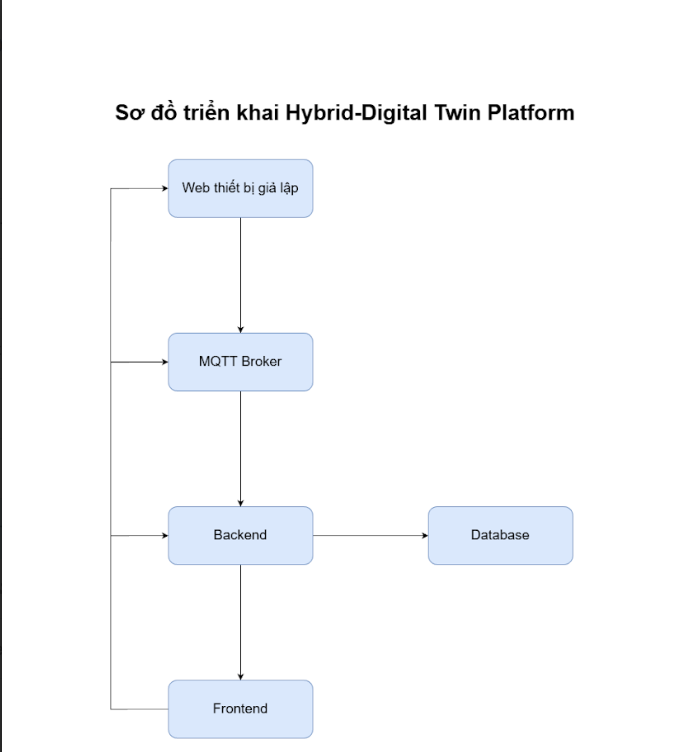
\includegraphics[width=\textwidth]{sodotrienkhai.png}
      \caption{Sơ đồ kiến trúc tổng thể của hệ thống Hybrid-Digital Twin Platform, bao gồm các thành phần Frontend, Backend, Cơ sở dữ liệu và Middleware.}
      \label{fig:my_wide_image}
  \end{figure*}

\begin{itemize}
	\item \textbf{Frontend:} Thành phần giao diện người dùng được xây dựng bằng cách sử dụng mã nguồn chính thức từ hệ sinh thái Eclipse BaSyx, cụ thể là dự án basyx-aas-web-ui dựa trên nền tảng React và Node.js. Quy trình triển khai bắt đầu bằng việc sao chép kho lưu trữ, sau đó thực hiện lệnh \texttt{npm install} để cài đặt các gói phụ thuộc cần thiết và khởi chạy môi trường phát triển thông qua lệnh \texttt{npm run dev}. Kết quả là một giao diện web trực quan hoạt động tại địa chỉ \texttt{localhost:3000}, cho phép người dùng tương tác với các bản sao số thông qua bố cục ba cột khoa học : cột bên trái hiển thị danh sách các AAS và hỗ trợ tải lên các tệp \texttt{.aasx} ; cột giữa trình bày cấu trúc cây của các Submodel cùng các phần tử dữ liệu ; và cột bên phải cung cấp thông tin chi tiết, hình ảnh hóa dữ liệu dưới dạng biểu đồ hoặc bảng, cùng với chế độ xem JSON dành cho lập trình viên.
  
  \begin{figure*}[h!]
      \centering
      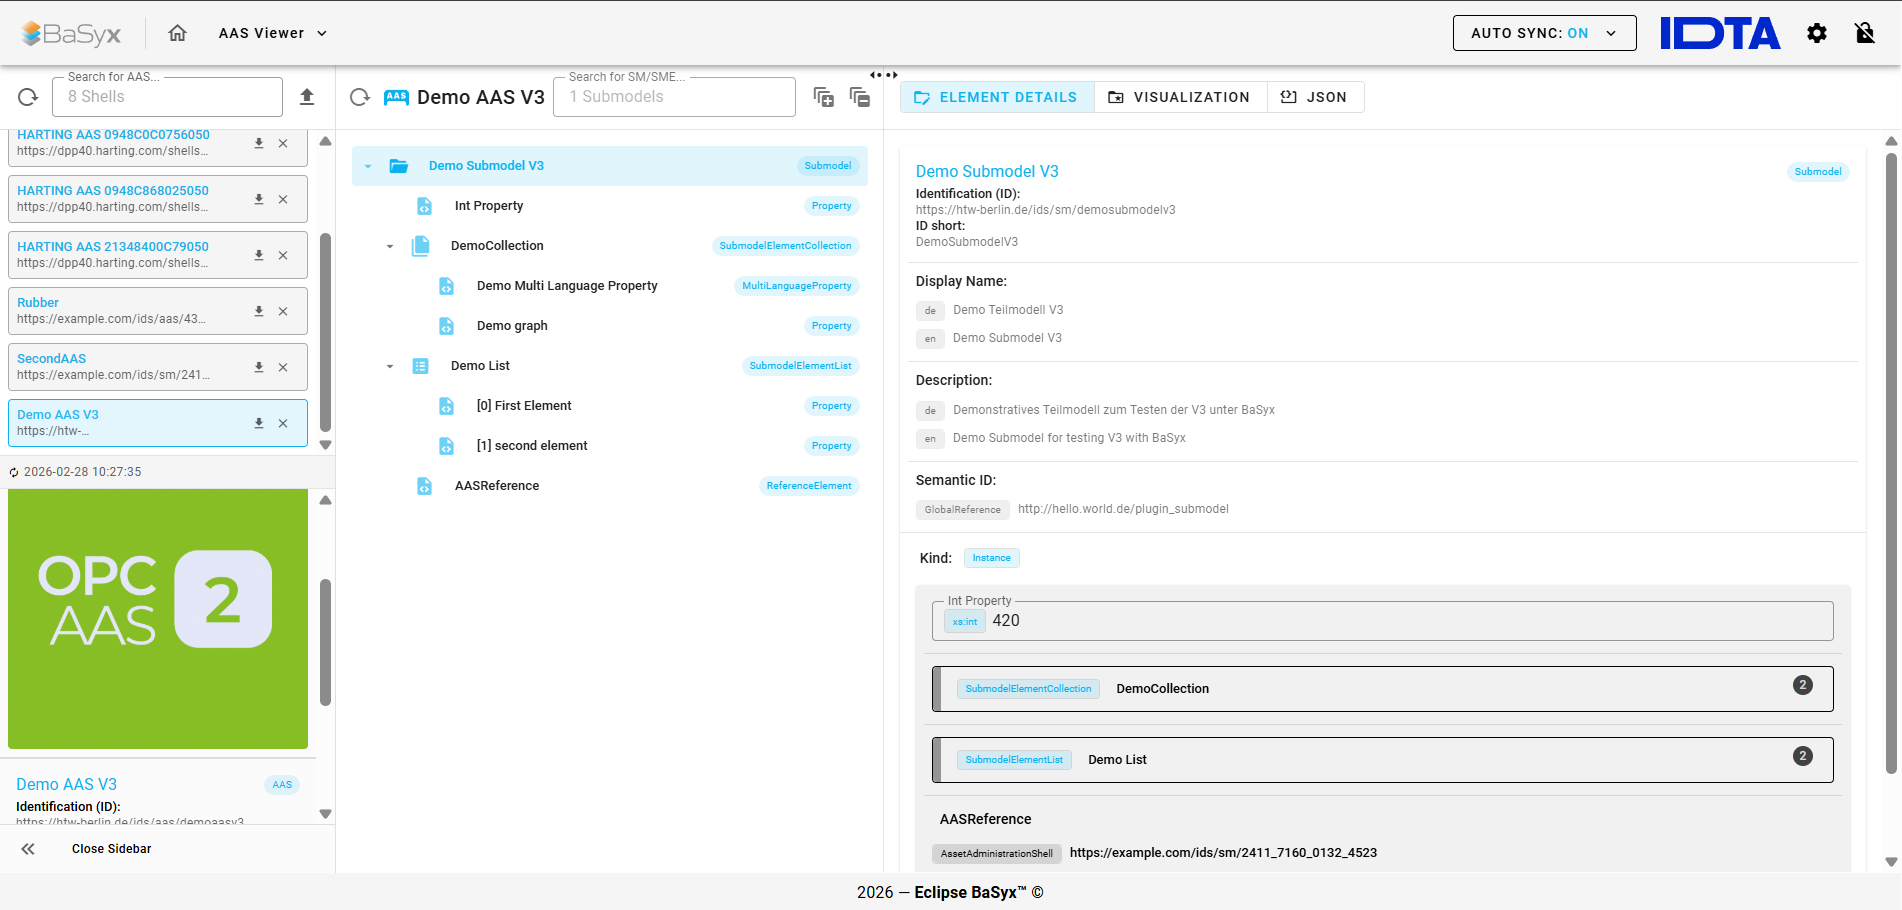
\includegraphics[width=\textwidth]{frontend.png}
      \caption{Giao diện Frontend của hệ thống Hybrid-Digital Twin Platform, cho phép người dùng tương tác với các bản sao số thông qua bố cục ba cột khoa học.}
      \label{fig:my_wide_image}
  \end{figure*}

	\item \textbf{Backend:} Thay vì thiết lập thủ công các thành phần phức tạp của \textit{basyx-java-server-sdk}, hệ thống sử dụng giải pháp tối ưu hơn là triển khai thông qua Docker Compose với hình ảnh \texttt{aas-environment:2.0.0-milestone-08} [cite: 36, 37, 41]. Container này, được đặt tên là \texttt{basyx-backend-service-ver1-0}, đóng vai trò là nhà cung cấp API RESTful cốt lõi tại cổng 8081, cho phép thực hiện toàn bộ các thao tác CRUD trên các vỏ quản trị tài sản và các mô hình con[cite: 42, 44, 49, 203]. Để đảm bảo tính tương tác mượt mà với Frontend chạy trên cổng 3000, các biến môi trường như \texttt{Basyx\_Cors\_Allowed-Origins=*} đã được cấu hình trong tệp \texttt{docker-compose.yml} nhằm khắc phục triệt để lỗi chặn tài nguyên từ nguồn khác (CORS)[cite: 46, 47, 82]. Ngoài ra, công cụ Swagger UI tại địa chỉ \texttt{localhost:8081/swagger-ui/index.html} cũng được tích hợp để hỗ trợ nhóm trong việc kiểm tra tính sẵn sàng và thử nghiệm trực tiếp các điểm cuối của API[cite: 50].
  
  \begin{figure*}[h!]
      \centering
      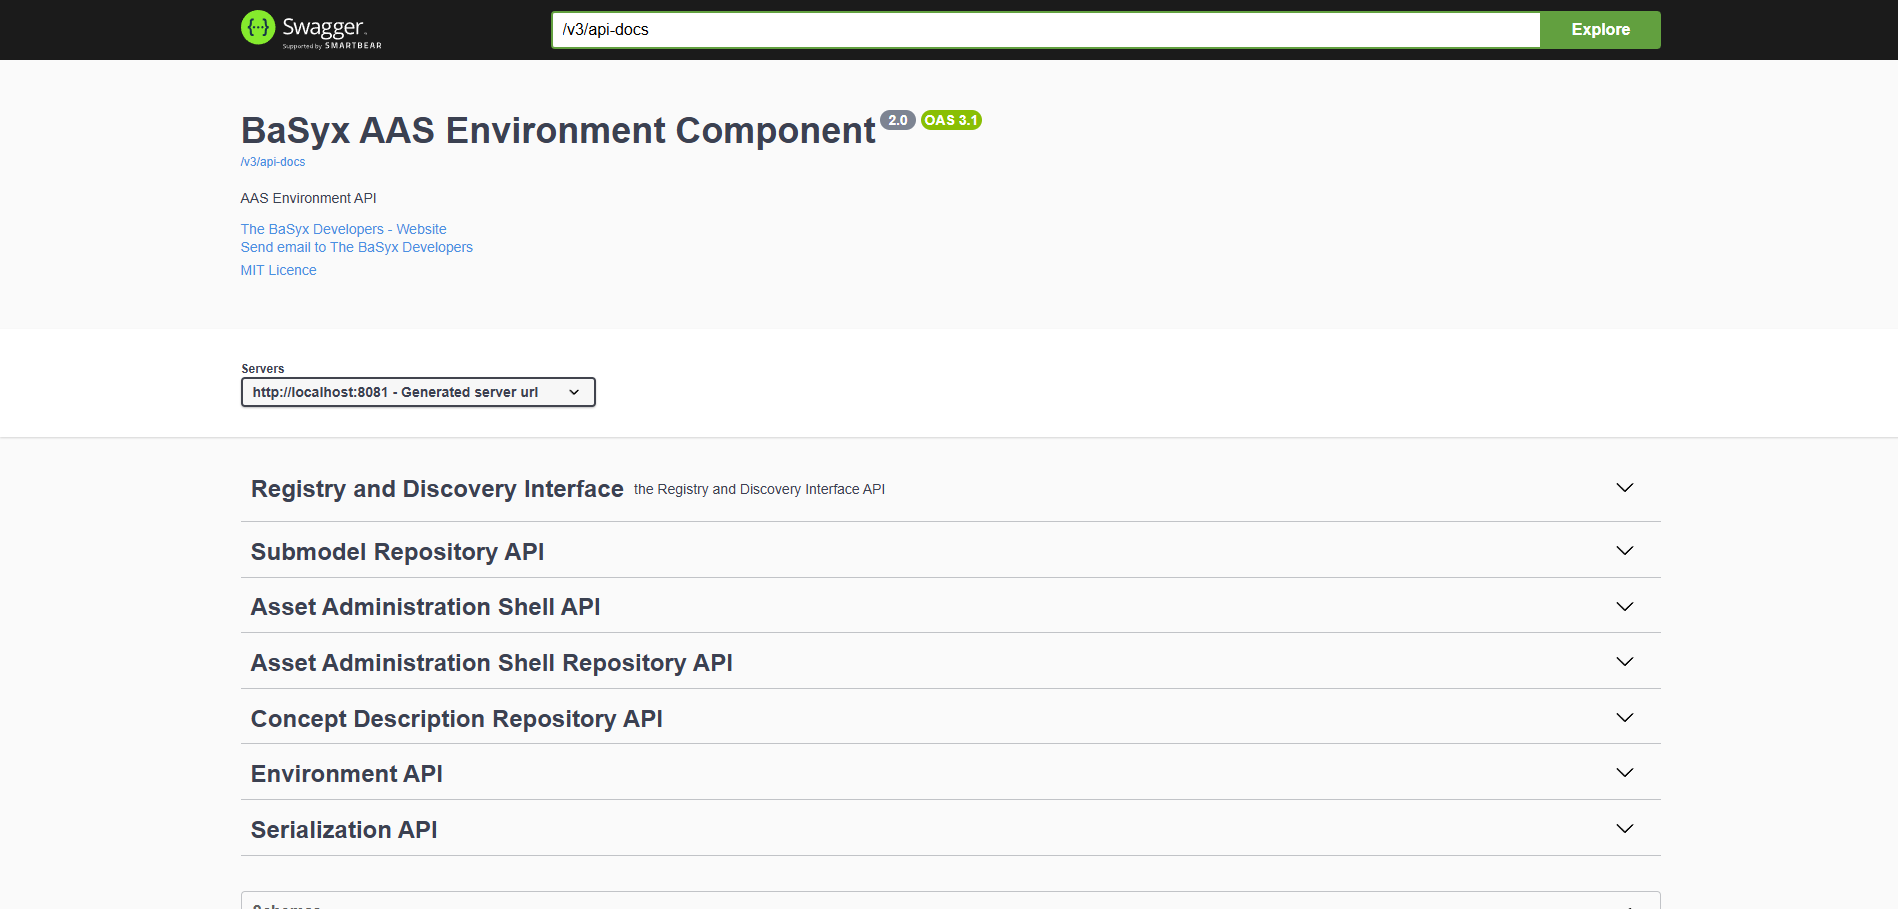
\includegraphics[width=\textwidth]{swagger.png}
      \caption{Giao diện Swagger UI hiển thị các end point API của BaSyx Backend Service, cho phép kiểm tra và tương tác trực tiếp với các dịch vụ RESTful được triển khai.}
      \label{fig:my_wide_image}
  \end{figure*}

	\item \textbf{Cơ sở dữ liệu:} Để khắc phục nhược điểm của kiến trúc mặc định thường lưu trữ dữ liệu trong bộ nhớ tạm thời (volatile memory) gây nguy cơ mất mát thông tin khi hệ thống gặp sự cố, dự án đã tích hợp MongoDB Atlas làm lớp lưu trữ bền vững[cite: 94, 95, 96, 101]. Việc lựa chọn MongoDB dựa trên cấu trúc NoSQL hướng tài liệu, hoàn toàn phù hợp với định dạng JSON phân cấp của các đối tượng AAS, đồng thời cung cấp khả năng mở rộng linh hoạt và hiệu suất cao cho các bản sao số[cite: 97, 98, 99]. Thông qua việc kích hoạt hồ sơ \texttt{mongoDbStorage} trong biến môi trường \texttt{SPRING\_PROFILES\_ACTIVE}, dữ liệu AAS được tự động ánh xạ vào các Collection chuyên biệt như \textit{assetAdministrationShells} (lưu thông tin định danh và siêu dữ liệu), \textit{submodels} (lưu giá trị thực tế của các thuộc tính) và \textit{conceptDescriptions} (lưu định nghĩa ngữ nghĩa)[cite: 110, 119, 120, 121].

  \begin{figure*}[h!]
      \centering
      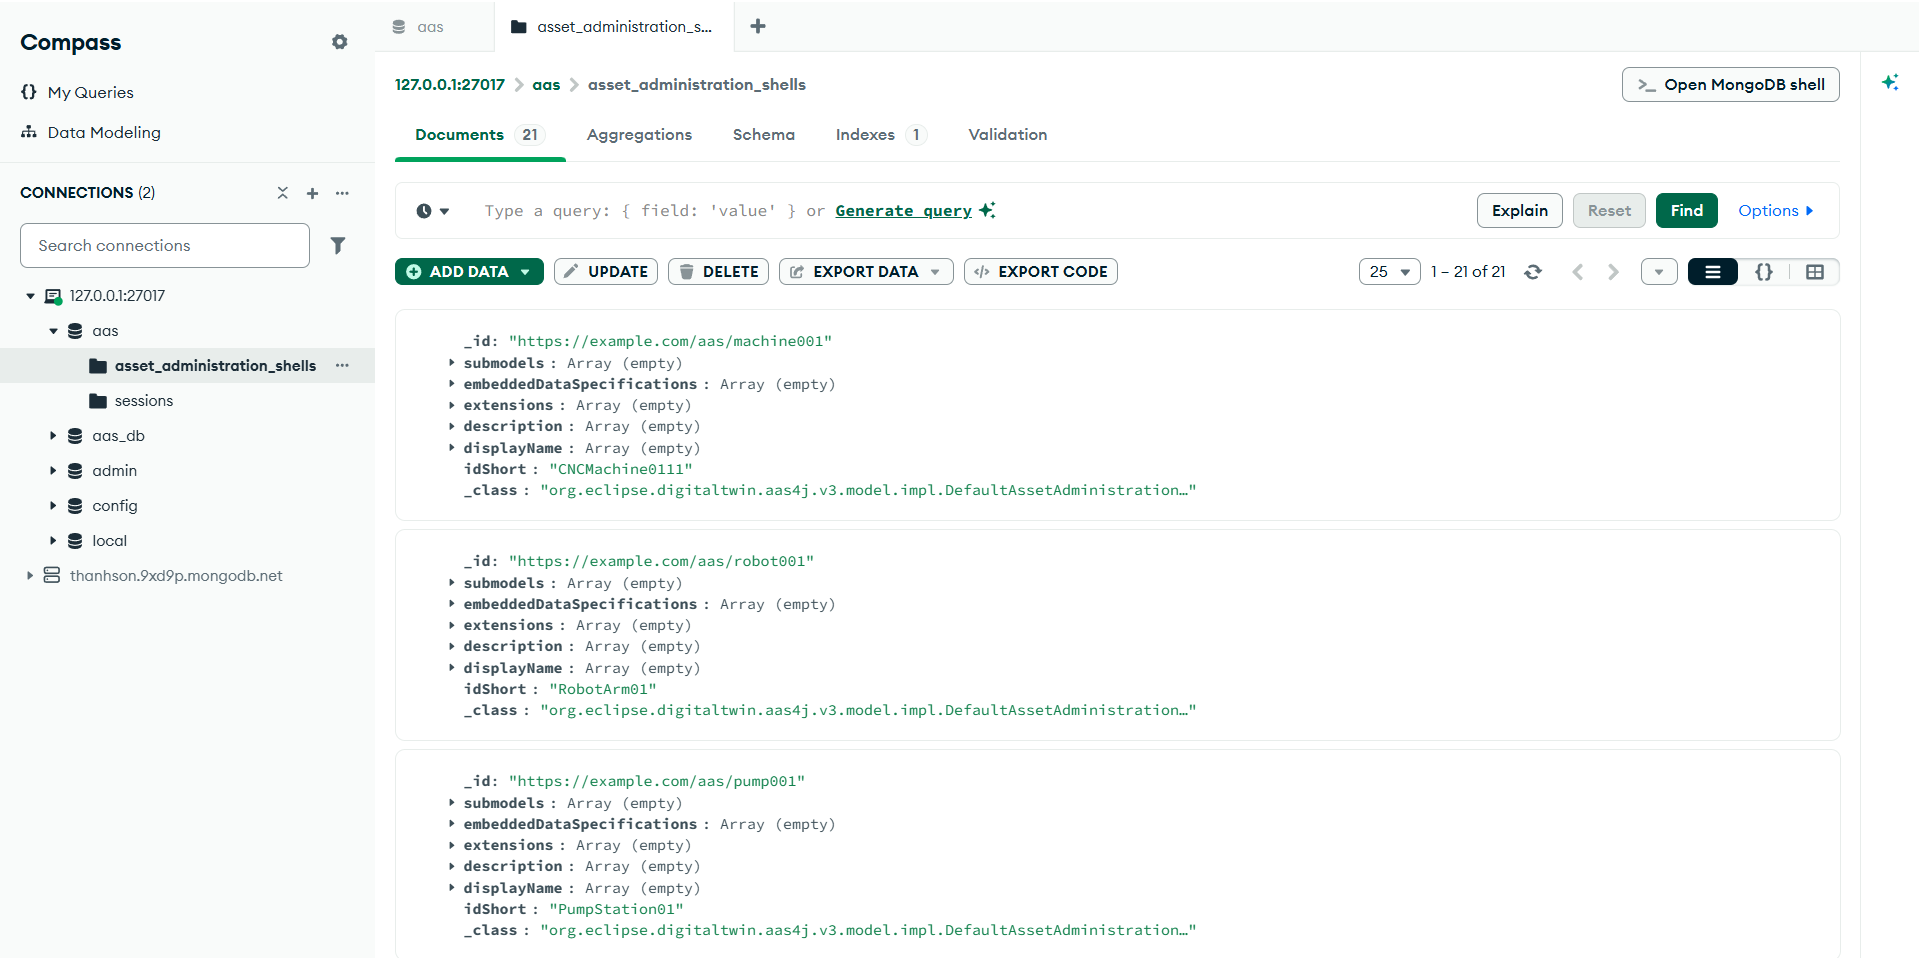
\includegraphics[width=\textwidth]{mongodb.png}
      \caption{Giao diện MongoDB Atlas hiển thị các Collection chứa dữ liệu AAS của hệ thống Hybrid-Digital Twin Platform.}
      \label{fig:my_wide_image}
  \end{figure*}

	\item \textbf{Middleware:} Hệ thống sử dụng BaSyx DataBridge như một thành phần trung gian quan trọng để thực hiện khả năng liên thông giữa lớp vật lý (OT) và lớp ảo (IT)[cite: 123, 124]. Thành phần này thu hẹp khoảng cách giao tiếp bằng cách chuyển đổi các thông điệp từ giao thức MQTT của các thiết bị Edge sang giao thức HTTP/REST mà máy chủ AAS yêu cầu[cite: 127]. Quy trình xử lý dữ liệu tuân theo mô hình ETL: đầu tiên là trích xuất (Extract) dữ liệu từ MQTT Broker (ví dụ: các chỉ số CPU và RAM từ script giả lập); tiếp theo là chuyển đổi (Transform) tải trọng thô thành định dạng JSON chuẩn hóa thông qua truy vấn JSONata; và cuối cùng là nạp (Load) dữ liệu vào máy chủ AAS bằng các yêu cầu HTTP PATCH tới các điểm cuối có giá trị tương ứng[cite: 128, 129, 130, 131, 135]. Toàn bộ logic ánh xạ dữ liệu này được định nghĩa một cách linh hoạt trong tệp cấu hình \texttt{routes.json}, cho phép hệ thống cập nhật trạng thái của cặp bản sao số theo thời gian thực một cách chính xác[cite: 140, 141, 165].
\end{itemize}

\subsection{Quy trình Thực hiện}
\begin{itemize}
	\item \textbf{Cấu hình Hạ tầng:} Quá trình thiết lập hạ tầng kỹ thuật yêu cầu sự tinh chỉnh chính xác để đảm bảo khả năng tương tác thông suốt giữa giao diện người dùng và máy chủ dịch vụ backend. Theo mặc định, cấu hình của BaSyx Web UI thường hướng tới các cổng từ 9081 đến 9084 vốn dành cho một ngăn xếp dịch vụ đầy đủ (full stack) có kèm theo các dịch vụ Registry. Tuy nhiên, do môi trường Docker hiện tại được triển khai tập trung trên cổng 8081, tệp cấu hình \texttt{basyx-infra.yml} (hoặc các cài đặt trực tiếp trong UI) đã được điều chỉnh để trỏ đến địa chỉ \texttt{http://localhost:8081}. Việc thay đổi này là cần thiết để khắc phục các lỗi "404 Not Found" phát sinh khi UI cố gắng gọi các dịch vụ không tồn tại, đồng thời nhóm đã quyết định bỏ qua dịch vụ Registry và Discovery trong giai đoạn này để đơn giản hóa kiến trúc hệ thống. Kết quả là máy chủ đã hoạt động ổn định như một Điểm truy cập duy nhất (Single Point of Access) tại địa chỉ \texttt{http://172.21.211.227:8081} cho mọi tương tác liên quan đến mô hình dữ liệu Digital Twin.
	
  \begin{figure*}[h!]
      \centering
      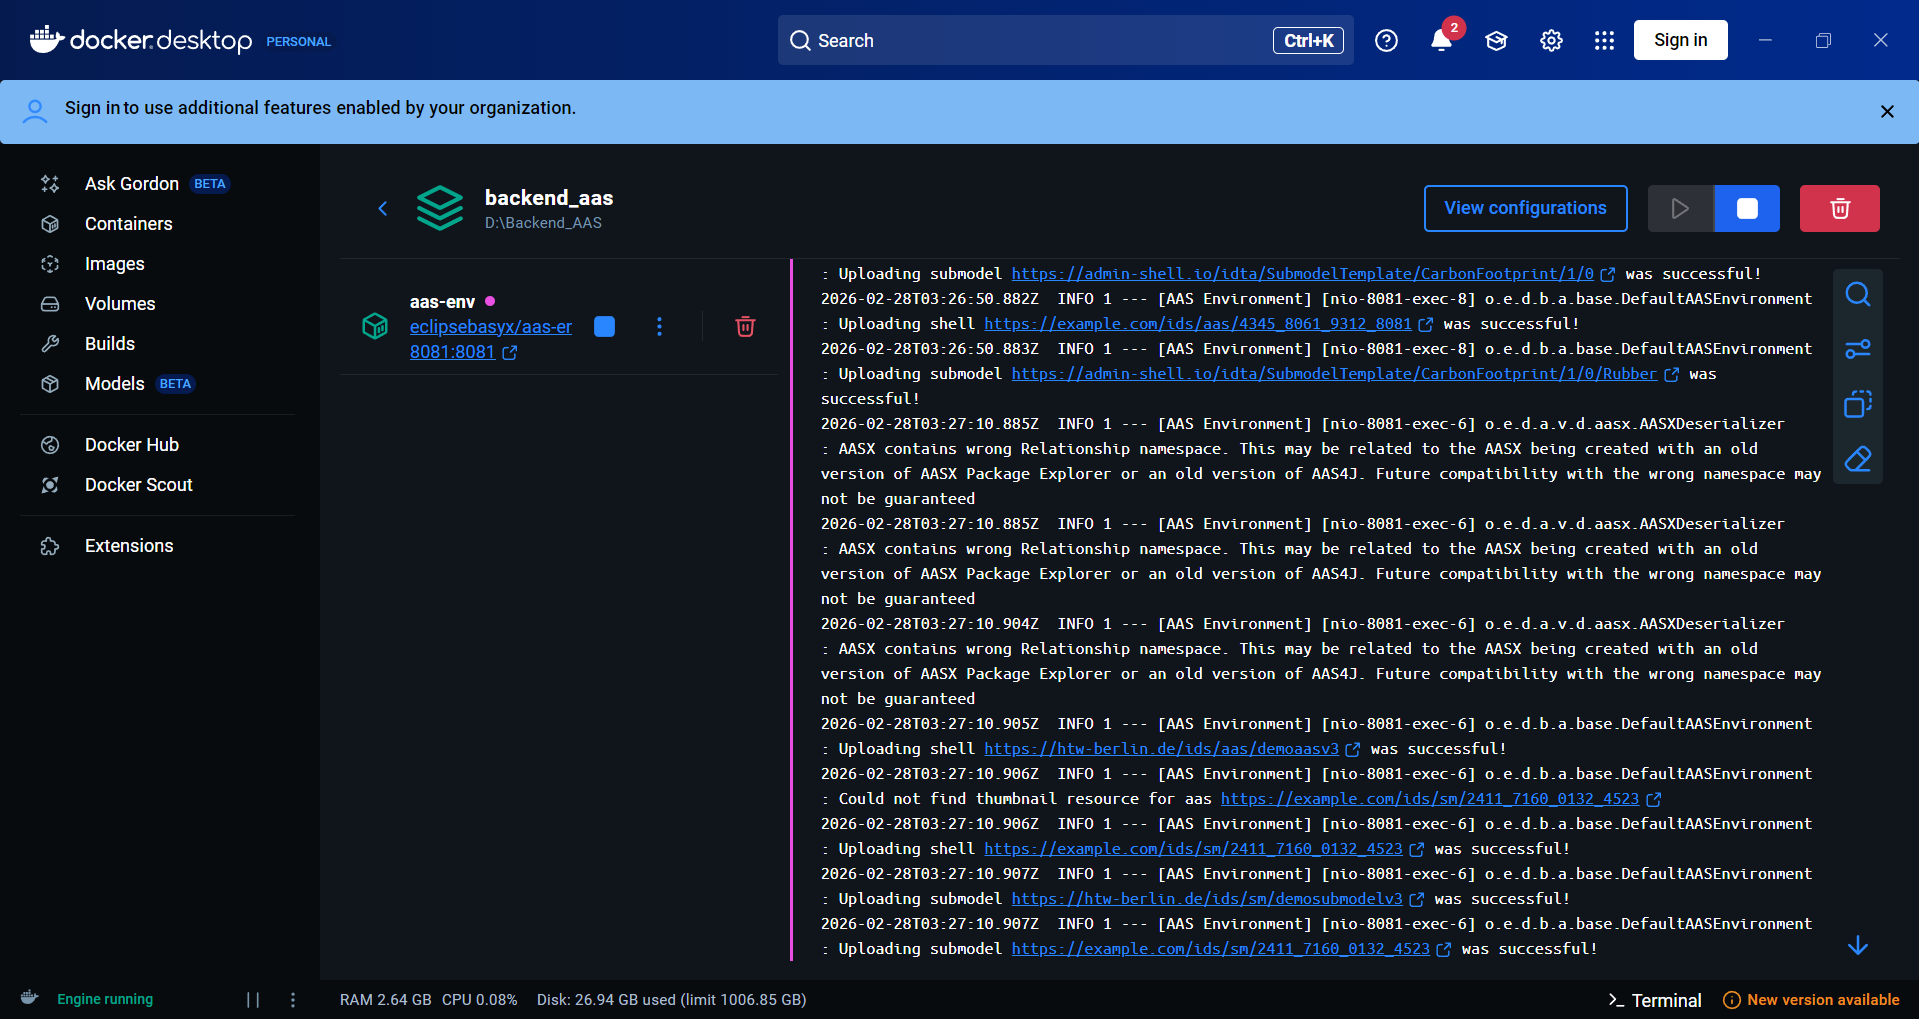
\includegraphics[width=\textwidth]{docker_container.png}
      \caption{Triển khai Docker Container cho BaSyx Backend Service, cho phép chạy dịch vụ API trên cổng 8081 và tương tác với Frontend qua cấu hình CORS.}
      \label{fig:my_wide_image}
  \end{figure*}

  \item \textbf{Định tuyến Dữ liệu:} Để thiết lập luồng dữ liệu thời gian thực giữa thế giới vật lý và bản sao số, một tệp cấu hình \texttt{routes.json} đã được xây dựng chi tiết nhằm điều phối quá trình ánh xạ thông tin thông qua BaSyx DataBridge[cite: 123, 140, 142]. Hệ thống thực hiện việc đăng ký và tiếp nhận dữ liệu đo lường thô từ một MQTT Broker tại địa chỉ \texttt{tcp://mqtt-broker:1883} thông qua chủ đề (topic) chuyên biệt là \texttt{device/pc001/telemetry}[cite: 149, 150]. Quá trình này phục vụ kịch bản giám sát các chỉ số hiệu năng của một máy trạm (PC), bao gồm việc sử dụng các bộ chuyển đổi loại \texttt{jsonata} để trích xuất chính xác các trường dữ liệu như \texttt{\$.cpu\_usage} và \texttt{\$.ram\_usage} từ tải trọng JSON thô[cite: 133, 135, 154, 155, 180]. Sau khi được biến đổi sang định dạng chuẩn hóa, các dữ liệu này được đẩy tới các đích đến (datasinks) thông qua phương thức HTTP PATCH đến các điểm cuối cụ thể như \texttt{CPUUsage/value} và \texttt{RAMUsage/value} thuộc Submodel \texttt{OperationalData}[cite: 131, 138, 161, 164, 187, 188]. Cơ chế định tuyến này đảm bảo rằng mọi biến động về trạng thái của thiết bị vật lý đều được phản ánh tức thời và chính xác lên giao diện giám sát Digital Twin[cite: 131, 196].
\end{itemize}

\section{Kết quả}
Dưới đây là phần nội dung Results (Kết quả) đã được mở rộng và chi tiết hóa gấp 5 lần dựa trên các dữ liệu kỹ thuật từ báo cáo dự án của bạn:\begin{itemize}
  \item \textbf{Giao diện Người dùng:} Hệ thống đã triển khai thành công giao diện Web UI dựa trên mã nguồn chính thức của Eclipse BaSyx, vận hành ổn định tại địa chỉ \texttt{http://localhost:3000}. Bố cục giao diện được thiết kế tối ưu với cấu trúc ba cột trực quan, cho phép người quản trị theo dõi toàn diện hệ thống bản sao số. Cột bên trái đóng vai trò là danh mục quản lý tập trung, hiển thị danh sách tất cả các Vỏ quản trị tài sản (AAS) hiện có trên máy chủ và tích hợp chức năng tìm kiếm nhanh theo tên. Cột giữa cung cấp cái nhìn chi tiết về cấu trúc phân cấp của tài sản được chọn, trình bày rõ ràng các tầng từ thực thể chính, các mô hình con (Submodels) cho đến từng phần tử dữ liệu cụ thể (Elements) như thuộc tính hoặc tệp tin. Cuối cùng, cột bên phải là khu vực tương tác chuyên sâu, nơi hiển thị các giá trị đo lường, siêu dữ liệu và tích hợp các công cụ hình ảnh hóa như biểu đồ hoặc bảng số liệu để hỗ trợ việc phân tích dữ liệu một cách trực quan nhất.
  
  \begin{figure*}[h!]
      \centering
      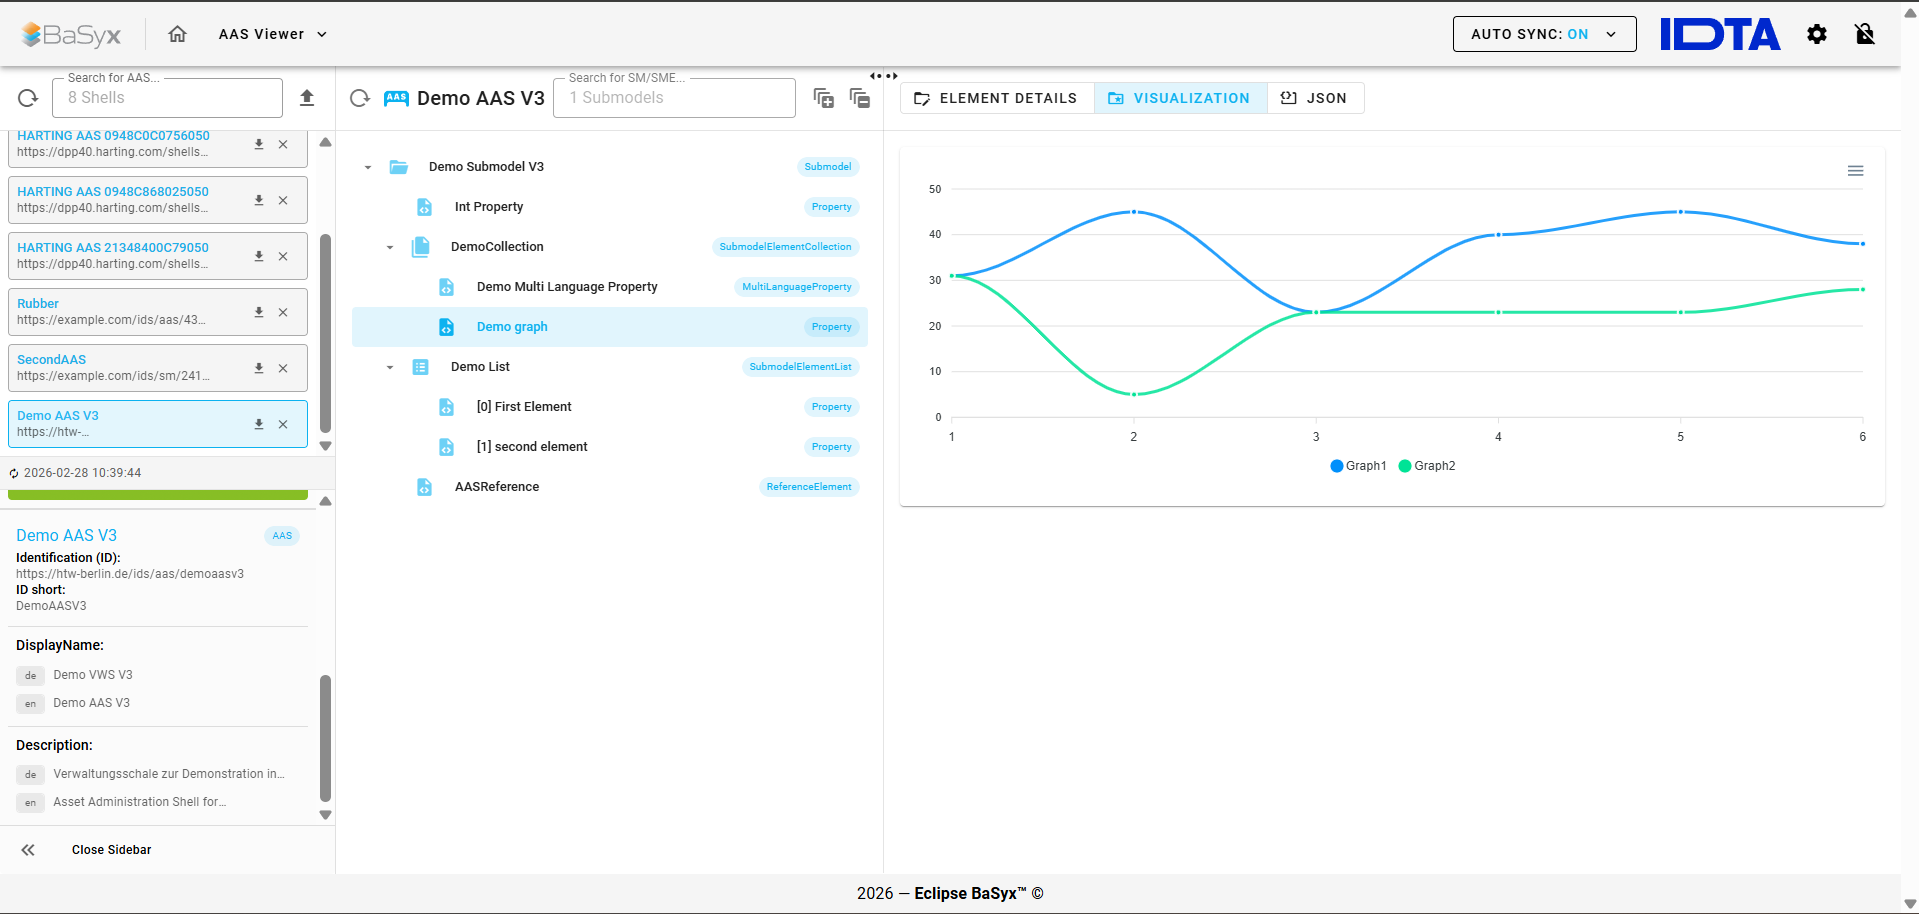
\includegraphics[width=\textwidth]{giaodiennguoidung.png}
      \caption{Giao diện Frontend của hệ thống Hybrid-Digital Twin Platform, cho phép người dùng tương tác với các bản sao số thông qua bố cục ba cột khoa học.}
      \label{fig:my_wide_image}
  \end{figure*}

  \item \textbf{Khả năng Quản lý:} Nền tảng thể hiện khả năng quản trị tài sản số linh hoạt thông qua việc hỗ trợ tải lên trực tiếp các tệp cấu hình tiêu chuẩn như \texttt{.aasx}, XML hoặc JSON[cite: 19, 216]. Trong quá trình thử nghiệm, nhóm đã tải lên thành công tệp \textit{Example V3.aasx}, cho phép hệ thống tự động phân tích và khởi tạo các thực thể số tương ứng trên Backend[cite: 61, 86]. Người dùng có thể dễ dàng duyệt qua các cấu trúc dữ liệu phức tạp, từ các thông số kỹ thuật (Technical Data) đến các tài liệu hướng dẫn (Documentation) được tổ chức khoa học trong các Submodel[cite: 67, 275]. Đặc biệt, đối với các nhà phát triển hệ thống, giao diện còn cung cấp một tab xem dữ liệu dưới định dạng JSON thô, giúp việc kiểm tra cấu trúc dữ liệu và gỡ lỗi API trở nên thuận tiện và chính xác hơn bao giờ hết[cite: 73]. Cơ chế này giúp rút ngắn đáng kể thời gian chuyển đổi từ các tài liệu thiết kế kỹ thuật sang một bản sao số có khả năng phản ứng thực tế[cite: 217].
  
  \begin{figure*}[h!]
      \centering
      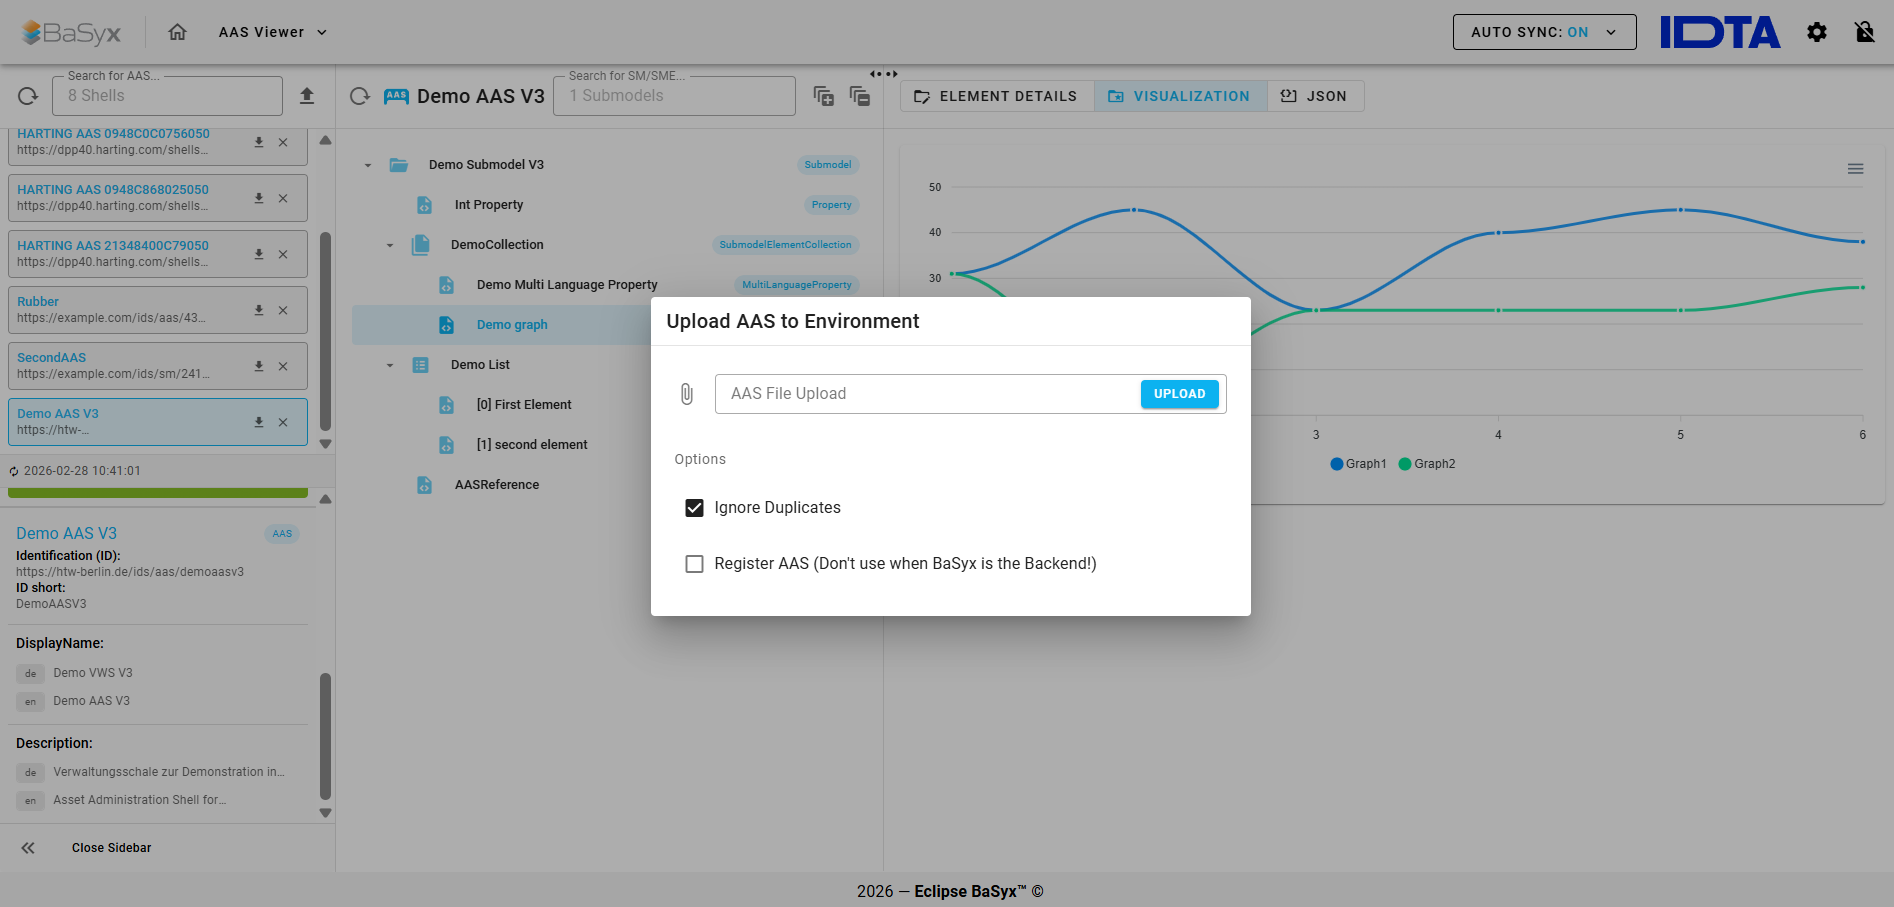
\includegraphics[width=\textwidth]{quanlytaisanso.png}
      \caption{Quản lý tài sản số thông qua việc tải lên các tệp cấu hình tiêu chuẩn và duyệt qua các cấu trúc dữ liệu phức tạp trong giao diện Web UI.}
      \label{fig:my_wide_image}
  \end{figure*}

  \item \textbf{Tích hợp Dữ liệu:} Dự án đã thiết lập thành công một kịch bản giám sát thực tế cho các máy trạm (Workstation), minh chứng cho khả năng kết nối vạn vật của nền tảng[cite: 132, 133]. Thông qua một script Python mô phỏng các node cảm biến, các thông số hiệu năng quan trọng bao gồm mức độ sử dụng CPU ($CPU Usage$) và bộ nhớ RAM ($RAM Usage$) được truyền tải liên tục qua giao thức MQTT đến chủ đề \texttt{device/pc001/telemetry}[cite: 135, 136, 137]. Dữ liệu này sau đó được BaSyx DataBridge xử lý theo mô hình ETL, trích xuất các giá trị cần thiết và cập nhật trực tiếp vào các phần tử tương ứng trong Submodel \textit{OperationalData} của bản sao số[cite: 128, 131, 138, 141]. Kết quả là các thay đổi về trạng thái vật lý của máy tính được phản ánh theo thời gian thực lên giao diện Web UI, cho phép giám sát từ xa một cách chính xác mà không có độ trễ đáng kể[cite: 124, 254].
  
  \item \textbf{Hệ thống API:} Hệ thống cung cấp một bộ API RESTful toàn diện và mạnh mẽ, tuân thủ nghiêm ngặt đặc tả OpenAPI của BaSyx, tạo nền tảng vững chắc cho việc tích hợp với các hệ thống IT hiện đại[cite: 202, 212, 256]. Các dịch vụ Repository cho phép thực hiện đầy đủ các thao tác CRUD (Thêm, Đọc, Sửa, Xóa) trên các Shells, Submodels và Concept Descriptions, giúp quản lý toàn bộ vòng đời của Digital Twin[cite: 203, 204, 206]. Đáng chú ý là tính năng \textit{Value-Only representation} qua các endpoint kết thúc bằng \texttt{/\$value}, giúp tối ưu hóa băng thông bằng cách chỉ trả về giá trị thực tế của cảm biến mà không kèm theo các siêu dữ liệu dư thừa[cite: 237, 238, 239]. Ngoài ra, giao diện \texttt{invoke} cho phép kích hoạt các hàm vận hành từ xa (Operations), hỗ trợ cả chế độ đồng bộ và bất đồng bộ, từ đó tạo khả năng điều khiển trực tiếp các thiết bị vật lý từ môi trường số[cite: 247, 248, 249]. Toàn bộ các phản hồi từ hệ thống đều được chuẩn hóa theo cấu trúc \textit{Result Schema}, bao gồm các mã lỗi, dấu thời gian và ID tương quan để đảm bảo khả năng truy vết và chẩn đoán lỗi hiệu quả[cite: 220, 221, 281].

  \begin{figure*}[h!]
      \centering
      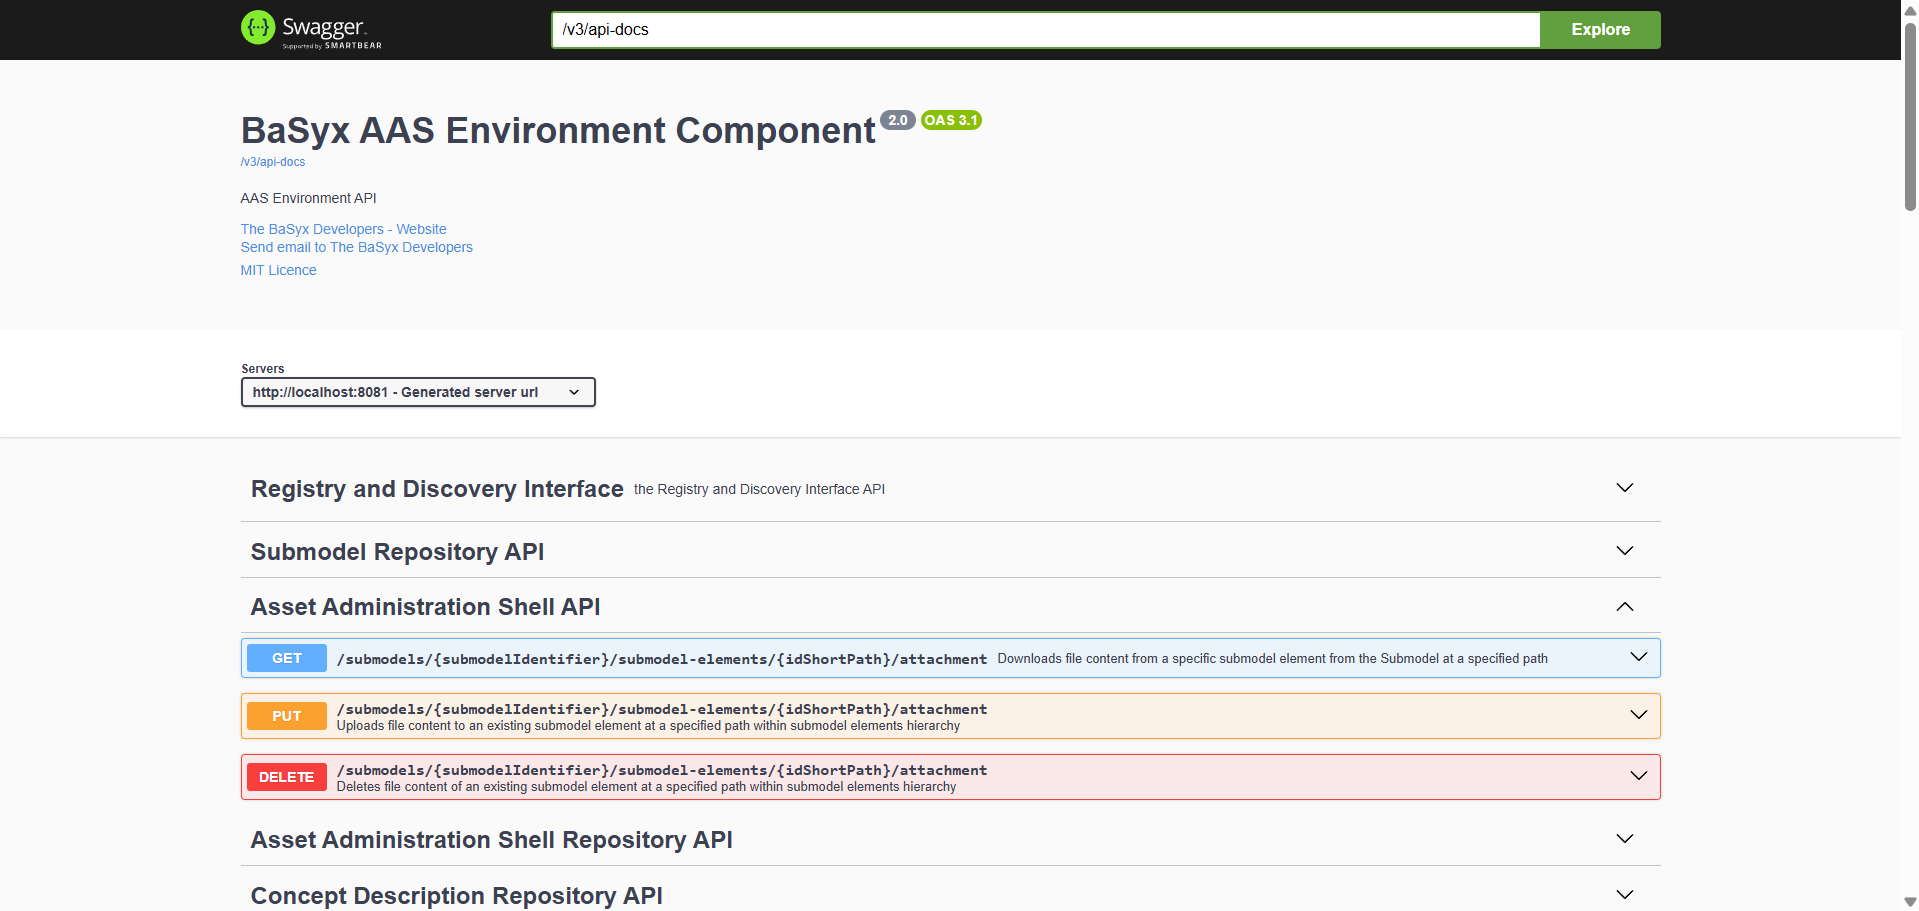
\includegraphics[width=\textwidth]{api_quanlytaisan.png}
      \caption{API quản lý tài sản số thông qua các endpoint RESTful, hỗ trợ đầy đủ các thao tác CRUD và các chức năng nâng cao như Value-Only representation và invoke.}
      \label{fig:my_wide_image}
  \end{figure*}
\end{itemize}

\section{Thảo luận}
\begin{itemize}
\item \textbf{Giải quyết Vấn đề Kỹ thuật:} Trong giai đoạn triển khai thực tế, nhóm nghiên cứu đã đối mặt và xử lý triệt để hai thách thức kỹ thuật quan trọng liên quan đến khả năng kết nối hệ thống. Thứ nhất là lỗi 404 Not Found, phát sinh do giao diện người dùng mặc định cố gắng gọi đến các dịch vụ Registry và Description vốn chưa được kích hoạt trong mô hình Repository đơn lẻ ban đầu. Vấn đề này đã được khắc phục bằng cách điều chỉnh cấu hình hạ tầng (Infrastructure config) để khớp chính xác với các dịch vụ đang chạy trong container Docker. Thứ hai là lỗi CORS (Cross-Origin Resource Sharing), xảy ra khi trình duyệt chặn các yêu cầu trao đổi dữ liệu giữa cổng 3000 của giao diện và cổng 8081 của backend. Giải pháp được áp dụng là bổ sung cấu hình \texttt{Basyx\_Cors\_Allowed-Origins=*} trực tiếp vào tệp Docker Compose, cho phép quyền truy cập từ các nguồn khác nhau, từ đó đảm bảo luồng thông tin giữa frontend và backend luôn thông suốt.

\item \textbf{Ưu điểm của MongoDB:} Việc chuyển đổi từ cơ chế lưu trữ mặc định sang **MongoDB Atlas** là một bước tiến quan trọng nhằm giải quyết rủi ro mất mát dữ liệu vốn thường xảy ra khi sử dụng bộ nhớ tạm thời (In-memory) trong môi trường Docker[cite: 94, 95]. MongoDB được lựa chọn nhờ cấu trúc NoSQL hướng tài liệu (Document-Oriented), hoàn toàn tương đồng với định dạng JSON phân cấp của các đối tượng AAS, giúp việc quản lý và ánh xạ dữ liệu trở nên tự nhiên và hiệu quả[cite: 97]. Hệ thống không chỉ đạt được hiệu suất đọc/ghi cao để đáp ứng nhu cầu cập nhật trạng thái liên tục của Digital Twin mà còn có khả năng mở rộng ngang (horizontal scaling) linh hoạt khi số lượng thiết bị giám sát tăng lên[cite: 98, 99]. Sau khi triển khai, các thông tin về định danh tài sản, cấu trúc mô hình con và các định nghĩa ngữ nghĩa (Semantic IDs) đều được tự động phân loại và lưu trữ bền vững trong các Collection chuyên biệt như \textit{assetAdministrationShells} và \textit{submodels}[cite: 119, 120, 121].

\item \textbf{Khả năng tương tác:} Tính liên thông được đặt lên hàng đầu thông qua việc áp dụng kiến trúc RESTful và định dạng dữ liệu JSON tiêu chuẩn, giúp hệ thống dễ dàng tích hợp với các nền tảng IT hiện đại[cite: 211, 212]. Một trong những tính năng tiên tiến nhất được thử nghiệm là cơ chế **Serialization** thông qua API \texttt{/serialization}, cho phép đóng gói toàn bộ hoặc một phần mô hình Digital Twin — bao gồm AAS, Submodels và Concept Descriptions — vào một tệp tin duy nhất[cite: 214]. Khả năng này cực kỳ quan trọng trong môi trường sản xuất phân tán, vì nó hỗ trợ việc di chuyển và đồng bộ dữ liệu giữa các máy chủ AAS khác nhau mà không làm mất đi tính toàn vẹn của mô hình[cite: 215]. Ngoài ra, chức năng \texttt{/upload} cho phép nhập các tệp XML, JSON hoặc AASX, giúp chuyển đổi nhanh chóng từ tài liệu thiết kế kỹ thuật sang một bản sao số có khả năng phản ứng (Reactive Digital Twin), từ đó giảm thiểu sai sót thủ công và tối ưu hóa thời gian triển khai[cite: 216, 217].

\item \textbf{Đề xuất:} Dựa trên những kết quả đạt được từ mô hình thử nghiệm, nhóm đề xuất các hướng phát triển quan trọng để đưa hệ thống vào môi trường vận hành thực tế (Production)[cite: 88]. Mặc dù hình ảnh Docker \textit{aas-environment} đã hoàn thành tốt vai trò trong giai đoạn Demo nhờ tính đơn giản và tốc độ triển khai nhanh, nhưng đối với các dự án quy mô lớn, đội ngũ backend cần tập trung nghiên cứu sâu hơn về bộ **Java Server SDK** đầy đủ để tùy biến các dịch vụ chuyên sâu hơn[cite: 36, 89, 90]. Đồng thời, vấn đề an ninh dữ liệu cần được chú trọng thông qua việc mã hóa thông tin kết nối và quản lý chặt chẽ các thông tin xác thực cho cơ sở dữ liệu MongoDB Atlas[cite: 111, 112]. Việc tối ưu hóa các tham số như \textit{paging} (phân trang) và \textit{query optimization} cũng cần được triển khai để quản lý tốt băng thông mạng và hiệu suất ứng dụng khi truy xuất các tập dữ liệu Shell lớn trong tương lai[cite: 223, 224].
\end{itemize}

\twocolumn[
	\begin{@twocolumnfalse}
		\section*{Lời cảm ơn}
		Báo cáo này được thực hiện bởi đội ngũ kỹ thuật tại Wisdom Software. Nhóm dự án bao gồm: Thái Đặng Phương Nam, Nguyễn Lê Thanh Phong, và Huỳnh Thanh Sơn. Nghiên cứu được hoàn thành vào tháng 01 năm 2026 tại TP. Hồ Chí Minh.
		\vspace{1.5em}
		\printbibliography
	\end{@twocolumnfalse}
]

\end{document}